\documentclass{beamer}
%\usecolortheme{dove} %Make title black
\usepackage{graphicx} % Allows including images
\usepackage{booktabs} % Allows the use of \toprule, \midrule and \bottomrule in tables
%\usepackage{siunitx}  %Use SI unit formatting
%\sisetup{range-phrase=--}
%Bold command
%\newcommand\SEC[1]{\textbf{\uppercase{#1}}}
\usepackage{pifont}% http://ctan.org/pkg/pifont
\newcommand{\cmark}{\ding{51}}%
\newcommand{\xmark}{\ding{55}}%
%\usepackage{siunitx}  %Use SI unit formatting
%For drawing beam line
\include{tikz}
\usetikzlibrary{shapes.misc}
\usetikzlibrary{shapes,arrows,decorations.markings,shadows,positioning}
%Adjust width of slide
\newcommand\Wider[2][3em]{%
	\makebox[\linewidth][c]{%
		\begin{minipage}{\dimexpr\textwidth+#1\relax}
			\raggedright#2
		\end{minipage}%
	}%
}

\include{header}
\usebackgroundtemplate{\includegraphics[width=\paperwidth]{NormalANLMaroon.pdf}}
\title[PSI Talk]{Photoinjector simulations for the Argonne Wakefield Accelerator facility}
\author[Speaker]{Nicole Neveu}
\subtitle{}
\institute[ANL/IIT]{Argonne National Laboratory\\Illinois Institute of Technology}
\date{\today}

\logo{%
	\makebox[0.95\paperwidth]{%
		%\includegraphics[width=3cm,keepaspectratio]{IIT_logo}%
		\hfill%
		\includegraphics[width=3cm,keepaspectratio]{IIT_logo_blk}%
	}%
}

\setbeamertemplate{navigation symbols}{}

%------------------------------------------------------
\begin{document}
\setbeamertemplate{footline}{}
{
	\usebackgroundtemplate{\includegraphics[width=\paperwidth]{TitleANLMaroon}}
	\logo{%
		\makebox[0.95\paperwidth]{%
			\includegraphics[width=3cm,keepaspectratio]{IIT_logo}%
			\hfill%
			%\includegraphics[width=3cm,keepaspectratio]{IIT_logo_blk}%
		}%
	}
	\frame{\titlepage}
}

\setbeamertemplate{footline}[page number]{}	
	
% FRAME: overview
\begin{frame}
  \frametitle{Outline}
  \tableofcontents
\end{frame}
% ========================================
% main slides come here
% ========================================
\section{Facility Introduction}
%\begin{frame}
%  \frametitle{Before we start ...}
%\end{frame}

\begin{frame}[plain]
\frametitle{AWA Facility}
\Wider[4em]{
  \setlength{\leftmargin}{0.1cm}
  \begin{itemize}
    \item{Two photocathode guns and accompanying linacs}
    \begin{itemize}
      \item{\underline{\textbf{Drive Line}}: $Cs_2Te$ cathode, 6 linac cavities}
      \begin{itemize}
        \item{Charge 0.1-100nC}
        \item{Energy up to 70 MeV}
      \end{itemize}
      \item{\underline{\textbf{Witness Line}}: $Mg$ cathode, 1 linac cavity}
      \begin{itemize}
        \item{Charge 0.1-10nC}
        \item{Energy up to 15 MeV}
      \end{itemize}
    \end{itemize}
    \item{Current experiments include:}
    \begin{itemize}
      \item{Two Beam Acceleration (TBA)}
      \item{Dielectric accelerating and decelerating structure tests}
      \item{Emittance Exchange (EEX)}
      \item{Electron Radiography Imaging (ERI)}
      \item{Cathode Studies}
    \end{itemize}  
  \end{itemize}
}
\end{frame}

\begin{frame}
\frametitle{AWA Facility}
\includegraphics[width=0.49\linewidth]{./pics/drive_gun}\hfill\includegraphics[width=0.49\linewidth]{./pics/TBA_overhead}\\
\includegraphics[width=0.49\linewidth]{./pics/dielectrics}\hfill\includegraphics[width=0.49\linewidth]{./pics/EEX}
\end{frame}
%--------------------------------------------------------------------------------------------
\section{Gun Benchmark: ASTRA, GPT, OPAL-t}
\begin{frame}
  \frametitle{Benchmark: ASTRA, GPT, OPAL-t}
  \begin{itemize}
    \item{Motivated by code features and my inexperience}
    \item{Used RF and solenoid maps from AWA photocathode gun}
    \item{Used PITZ operating conditions as input parameters}
    \item{Poster presented at NAPAC'16: THPOA46}
    \item{Spoiler: No major differences found}
  \end{itemize}
\end{frame}

\begin{frame}
	%\def\checkmark{\tikz\fill[scale=0.4](0,.35) -- (.25,0) -- (1,.7) -- (.25,.15) -- cycle;} 
	\frametitle{Code Features}
	\begin{table}\centering
		\begin{tabular}{l l l l}
			\toprule
			\textbf{Feature} & \textbf{ASTRA} & \textbf{GPT} & \textbf{OPAL}\\
			\midrule
			Windows     		& \cmark & \cmark & \xmark \\ 
			Mac         		& \cmark & \cmark & \cmark \\
			Linux       		& \cmark & \cmark & \cmark \\
			Open Source 		& \xmark & \xmark & \cmark \\
			Parallel    		& \xmark\footnote[1]{A parallel version is available at DESY} & \xmark & \cmark \\
			Autophase   		& \cmark & \xmark & \cmark \\
			Adaptive Time Step 	& \xmark & \cmark & \xmark \\
			3D Space Charge 	& \cmark & \cmark & \cmark \\
			Wakefields  		& \cmark & \xmark\footnote[2]{In house module was written at AWA\label{note2}} & \cmark \\
			CSR         		& \xmark & \xmark\textsuperscript{\ref{note2}} & \cmark \\
			\bottomrule
		\end{tabular}
		%\caption{Table caption}
	\end{table}
\end{frame}

\begin{frame}
\frametitle{Model and Input Parameters}
\begin{minipage}{0.3\textwidth}
\def \gunleft {-1.0}
\def \gunright {0.3}
\def \loneright {1.0}
\def \ltworight {3.5}
\def \lthreeright {5.0}
\def \lfourright {7.0}
\def \lfiveright {8.5}
\def \lsixright {10}
        \begin{center}
                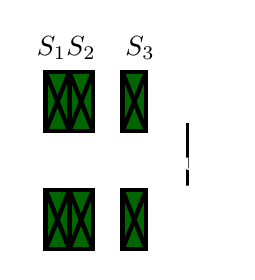
\begin{tikzpicture}[scale=0.75]
                %Gun drawings
                \draw[fill=orange, very thick, rounded corners =0.1cm] (\gunleft,0.5)rectangle (\gunright,1.5) node[pos=.5, white] {\textbf{Gun}} ;

                %S1
                \node[] at (-1.3,2.9) {$S_1$};
                \draw[ultra thick, fill=black!60!green] (-1.4,-0.5)rectangle  (-1.0,0.5) node[pos=.5, white] {} ;
                \draw[black, ultra thick] (-1.4,-0.5) -- (-1.0,0.5);
                \draw[black, ultra thick] (-1.4,0.5) -- (-1.0,-0.5);
                \draw[ultra thick, fill=black!60!green] (-1.4,1.5)rectangle  (-1.0,2.5) node[pos=.5, white] {} ;
                \draw[black, ultra thick] (-1.4,1.5) -- (-1.0,2.5);
                \draw[black, ultra thick] (-1.4,2.5) -- (-1.0,1.5);
                %S2
                \node[] at (-0.8,2.9) {$S_2$};
                \draw[ultra thick, fill=black!60!green] (-1.0,-0.5)rectangle  (-0.6,0.5) node[pos=.5, white] {} ;
                \draw[black, ultra thick] (-1.0,-0.5) -- (-0.6,0.5);
                \draw[black, ultra thick] (-1.0,0.5) -- (-0.6,-0.5);
                \draw[ultra thick, fill=black!60!green] (-1.0,1.5)rectangle  (-0.6,2.5) node[pos=.5, white] {} ;
                \draw[black, ultra thick] (-1.0,1.5) -- (-0.6,2.5);
                \draw[black, ultra thick] (-1.0,2.5) -- (-0.6,1.5);

                %S3
                \node[] at (0.2,2.9) {$S_3$};
                \draw[ultra thick, fill=black!60!green] (-0.1,-0.5) rectangle  (0.3,0.5) node[pos=.5, white] {};
                \draw[black, ultra thick] (-0.1,-0.5) -- (0.3,0.5);
                \draw[black, ultra thick] (-0.1,0.5) -- (0.3,-0.5);
                \draw[ultra thick, fill=black!60!green] (-0.1,1.5) rectangle  (0.3,2.5) node[pos=.5, white] {};
                \draw[black, ultra thick] (-0.1,1.5) -- (0.3,2.5);
                \draw[black, ultra thick] (-0.1,2.5) -- (0.3,1.5);
\end{tikzpicture}
\end{center}
\end{minipage} \hfill
\begin{minipage}{0.65\textwidth}
\begin{table}\centering
	\begin{tabular}{l c c}
		\toprule 
		\textbf{Parameter} & \textbf{Value} \\
		\midrule
		Charge  		& 1 nC \\
		$S_3$ 			&  -0.389 T \\
		$S_1$ and $S_2$ & -0.12 T \\
		Laser Radius 	& 0.75 mm \\
		Laser FWHM 		& 20 ps \\
		Laser Rise/Fall Time & 6 ps \\
		Gun Gradient 	& 60 MV/m \\
		Phase 			& Max Energy \\
		Kinetic Energy on Cathode & 0.55 eV \\
		\bottomrule
	\end{tabular}
\end{table}
\end{minipage}
\end{frame}


\begin{frame}
  \frametitle{Benchmark Results}
  \Wider[4em]{
  All codes matched within $5\%$. \\
  Well below measurement thresholds at AWA.\\  
  \vfill \vfill
  \includegraphics[width=0.49\linewidth]{wikitestNoMinStep}\hfill \includegraphics[width=0.49\linewidth]{wikitest5mNoMinStep}
}
\end{frame}

%--------------------------------------------------------------------------------------------
\section{Future Work with optPilot}
\begin{frame}
  \frametitle{OptPilot}
\end{frame}

\begin{frame}
  \frametitle{New beam line under design}
\Wider[4em]{
\def \gunleft {-1.0}
\def \gunright {0.3}
\def \loneright {1.0}
\def \ltworight {3.5}
\def \lthreeright {5.0}
\def \lfourright {7.0}
\def \lfiveright {8.5}
\def \lsixright {10}
        \centering
        \begin{center}
                \begin{tikzpicture}[scale=0.7]
                %Gun drawings
                \draw[fill=orange, very thick, rounded corners =0.1cm] (\gunleft,0.5)rectangle (\gunright,1.5) node[pos=.5, white] {\textbf{Gun}} ;

                %S1
                \node[] at (-1.3,2.9) {$S_1$};
                \draw[ultra thick, fill=black!60!green] (-1.4,-0.5)rectangle  (-1.0,0.5) node[pos=.5, white] {} ;
                \draw[black, ultra thick] (-1.4,-0.5) -- (-1.0,0.5);
                \draw[black, ultra thick] (-1.4,0.5) -- (-1.0,-0.5);
                \draw[ultra thick, fill=black!60!green] (-1.4,1.5)rectangle  (-1.0,2.5) node[pos=.5, white] {} ;
                \draw[black, ultra thick] (-1.4,1.5) -- (-1.0,2.5);
                \draw[black, ultra thick] (-1.4,2.5) -- (-1.0,1.5);
                %S2
                \node[] at (-0.8,2.9) {$S_2$};
                \draw[ultra thick, fill=black!60!green] (-1.0,-0.5)rectangle  (-0.6,0.5) node[pos=.5, white] {} ;
                \draw[black, ultra thick] (-1.0,-0.5) -- (-0.6,0.5);
                \draw[black, ultra thick] (-1.0,0.5) -- (-0.6,-0.5);
                \draw[ultra thick, fill=black!60!green] (-1.0,1.5)rectangle  (-0.6,2.5) node[pos=.5, white] {} ;
                \draw[black, ultra thick] (-1.0,1.5) -- (-0.6,2.5);
                \draw[black, ultra thick] (-1.0,2.5) -- (-0.6,1.5);

                %S3
                \node[] at (0.2,2.9) {$S_3$};
                \draw[ultra thick, fill=black!60!green] (-0.1,-0.5) rectangle  (0.3,0.5) node[pos=.5, white] {};
                \draw[black, ultra thick] (-0.1,-0.5) -- (0.3,0.5);
                \draw[black, ultra thick] (-0.1,0.5) -- (0.3,-0.5);
                \draw[ultra thick, fill=black!60!green] (-0.1,1.5) rectangle  (0.3,2.5) node[pos=.5, white] {};
                \draw[black, ultra thick] (-0.1,1.5) -- (0.3,2.5);
                \draw[black, ultra thick] (-0.1,2.5) -- (0.3,1.5);
                %Linac drawings 
                \draw[fill=blue, ultra thick, rounded corners =0.1cm] (\loneright,0)rectangle  ({\loneright+0.84},2) node[pos=.5, white] {$L_1$} ;
                \draw[fill=blue, ultra thick, rounded corners =0.1cm] (\ltworight,0)rectangle  ({\ltworight+0.84},2) node[pos=.5, white] {$L_2$};
                \draw[fill=blue, ultra thick, rounded corners =0.1cm] (\lthreeright,0)rectangle ({\lthreeright+0.84},2) node[pos=.5, white] {$L_3$};
                \draw[fill=blue, ultra thick, rounded corners =0.1cm] (\lfourright,0)rectangle ({\lfourright+0.84},2) node[pos=.5, white] {$L_4$};
                \draw[fill=blue, ultra thick, rounded corners =0.1cm] (\lfiveright,0)rectangle ({\lfiveright+0.84},2) node[pos=.5, white] {$L_5$};
                \draw[fill=blue, ultra thick, rounded corners =0.1cm] (\lsixright,0)rectangle ({\lsixright+0.84},2) node[pos=.5, white] {$L_6$};
                 
                %current optimization point
                %\node[draw, fill=yellow, star, star points=5, star point ratio=0.6, minimum size=0.1cm]
                %at (12.5,1.0) {$z_1$};


                %Quad drawings
                %\draw[fill=black!60!green] (12.52, 1.0) ellipse (0.3cm and 0.9cm);
                %\draw[fill=black!60!green] (13.28, 1.0) ellipse (0.3cm and 0.9cm);

                \draw[very thick] (\gunleft,-5.0) -- (14,-5.0);
                \draw[latex-latex] (\gunleft,-5.0) -- (14,-5.0) ;
                \foreach \x in  {0.3, 1.0, 3.5, 5.0, 7.0, 8.5, 10, 12.5} %tick marks
                \draw[shift={(\x,-5.0)},color=black] (0pt,3pt) -- (0pt,-3pt);
                \foreach \x in {0.3, 1.0, 3.5, 5.0, 7.0, 8.5, 10, 12.5}
                \draw[shift={(\x,-5.2)},color=black] (0pt,0pt) node[below] {$\x$};

                \end{tikzpicture}
   \end{center}
}
\end{frame}

%--------------------------------------------------------------------------------------------
\section{Initial Python Optimization Results}


\end{document}









